% !TEX root = ../../main.tex
\chapter{Signal Region Optimizations}
\label{ch:opt}

Several optimizations of the event selection have been implemented with respect to the previous Run-II analysis (13.2\,\ifb)~\cite{ichep2016supportnote, lvqq_conf_2016}. In~\Sect{\ref{ch:opt:newlp}}, a new low purity (LP) signal region (SR) definition is studied. In~\Sect{\ref{ch:opt:vbf}}, the method of selecting VBF jets is explored, for the new VBF selection. In~\Sect{\ref{sec:TAmass}}, the improvement offered by the track assisted mass in the high-\pT region is verified. 



%Add VBF mjj vs dy?

%
\section{Low Purity Signal Region Definition}
\label{ch:opt:newlp}
The LP SR has been updated to include the 80\,\% $V$-tagging efficiency working points of the SmoothedWZTagger. The updated definition is intended to increase the sensitivity of the search, and to harmonize the signal regions with other diboson search channels at ATLAS. The two definitions are summarized below:
\begin{itemize}
\item\underline{New}: Large-R jet must fail {\em at least one} 50\,\% efficiency working point (i.e. mass window, $D_2^{\beta=1}$ upper cut, or both). Additionally, the large-R jet must pass {\em both} the 80\,\% efficiency mass window working point and the 80\,\% efficiency $D_2^{\beta=1}$ working point.
\item\underline{Old}: Large-R jet must pass the 50\,\% efficiency mass window working point, and fail the 50\,\% efficiency $D_2^{\beta=1}$ working point.
\end{itemize}

To quantify the sensitivity of the two LP SR definitions, the significance around signal mass points are calculated. A window of $\pm2\sigma_m$ from the center of the signal mass distribution is used. The significance is then evaluated as:
$$\sigma_{sig}=\sqrt{2\times(s+b)\times\log\left(1+\frac{s}{b}\right) - 2s}$$
Where $s$ is the number of signal events, and $b$ is the number of background events passing the selection.

In~\Fig{\ref{fig:lp_sr_def}}, the significance is plotted as a function of resonance mass for both VBF and ggF selections. For both the VBF and ggF selection, a scalar heavy Higgs (NWA) model is used for signal masses ranging from 500\,\GeV\, to 3\,\TeV. In all cases, the new definition of the LP SR increases the sensitivity of the search. Since the HP SR is prioritized, changing the LP SR definition while leaving the HP SR definition unchanged does not affect the sensitivity of the HPSR.

\begin{figure}[tbp]
\centering
\subfloat[]{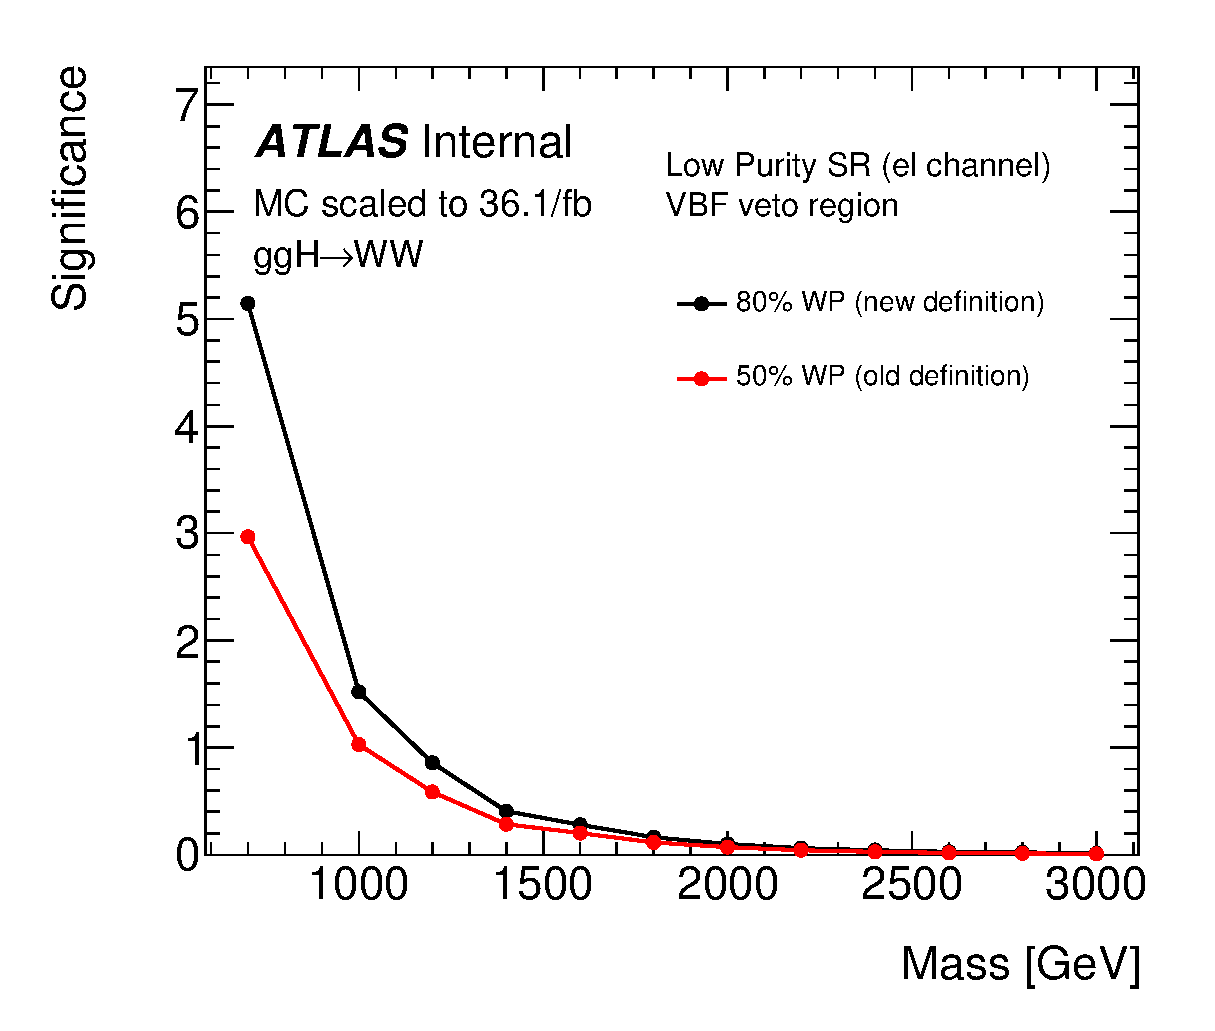
\includegraphics[width=.48\textwidth]{figures/Appendix/opt/WZtag/comp_ggf_sig_ggf_reg_el}\label{fig:lp_sr_def:a}}
\subfloat[]{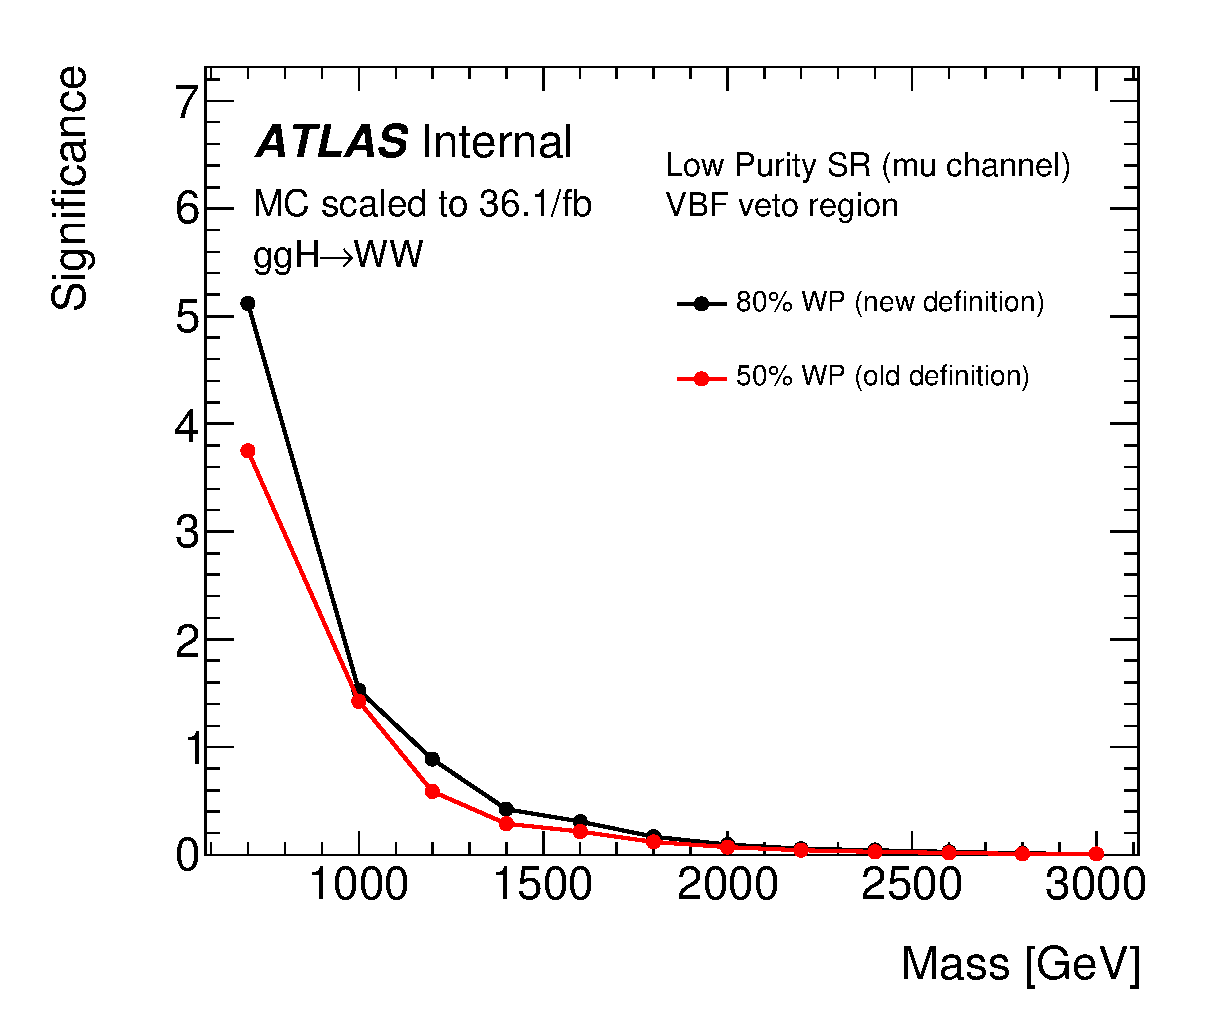
\includegraphics[width=.48\textwidth]{figures/Appendix/opt/WZtag/comp_ggf_sig_ggf_reg_mu}\label{fig:lp_sr_def:b}}\\
\subfloat[]{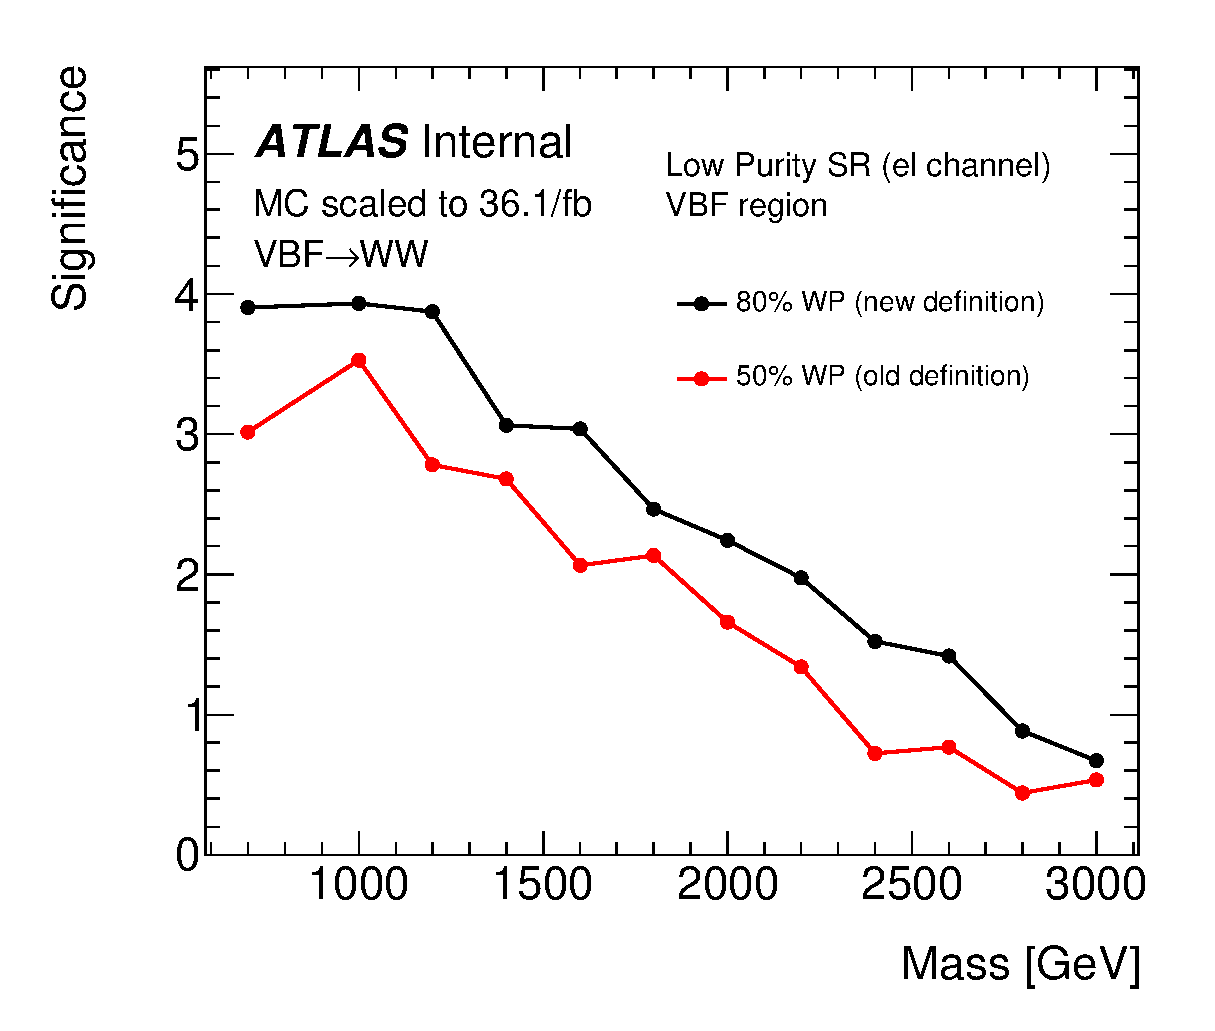
\includegraphics[width=.48\textwidth]{figures/Appendix/opt/WZtag/comp_vbf_sig_vbf_reg_el}\label{fig:lp_sr_def:c}}
\subfloat[]{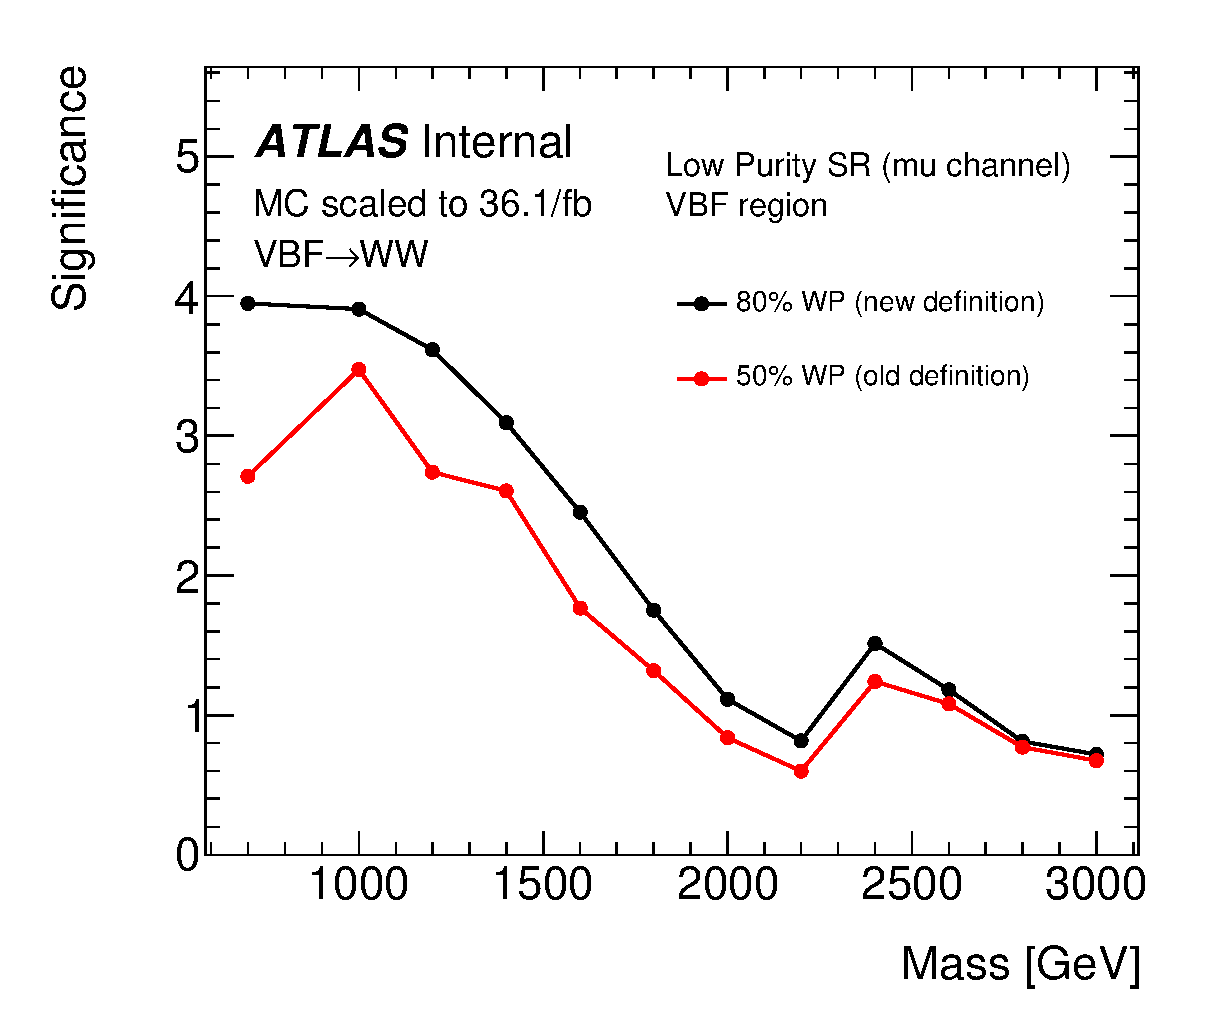
\includegraphics[width=.48\textwidth]{figures/Appendix/opt/WZtag/comp_vbf_sig_vbf_reg_mu}\label{fig:lp_sr_def:d}}
\caption[Low purity region definition optimization]{The gain in sensitivity due to the new LP SR definition is illustrated. The LP SR definitions for the ggF selection is shown for the \protect\subref{fig:lp_sr_def:a} $e$-channel  and \protect\subref{fig:lp_sr_def:b} $\mu$-channel. The LP SR definitions for the VBF selection is shown for the \protect\subref{fig:lp_sr_def:c} $e$-channel and \protect\subref{fig:lp_sr_def:d} $\mu$-channel. For both ggF and VBF selections, a heavy scalar Higgs (NWA) model was used, for masses between 500\,\GeV\, and 3\,\TeV.}
\label{fig:lp_sr_def}
\end{figure}

%
\clearpage
\section{Selection of  Vector Boson Fusion Jets}
\label{ch:opt:vbf}
In the newly added VBF selection, there were two proposed methods to select the small-R jets from the initial quarks radiating vector bosons.  The updated definition was introduced to harmonize the selection with other diboson search channels at ATLAS. The two definitions are summaried below:
\begin{itemize}
\item\underline{$m^{\rm VBF}(j,j)$}: Select pair of small-R jets with the largest invariant mass first, $m^{\rm VBF}(j,j)$. Then select the large-R jet (if any) for the boosted hadronic decay, provided the large-R jet does not overlap with either VBF-tagged small-R jet. Finally, the rest of the VBF selections are applied.
\item\underline{Highes $\pT(j)$}: The large-R jet is selected first. Then, VBF jets are selected by finding the two small-R jets with the highest $\pT$. Finally, the rest of the VBF selections are applied.
\end{itemize}

The sensitivity of both definitions is quantified using the significance definition described in~\Sect{\ref{ch:opt:newlp}}. In~\Fig{\ref{fig:mjj_comb}}, the combined HP SR and LP SR is shown for both VBF selections. In~\Fig{\ref{fig:mjj_lp}}, the sensitivity for just the LP SR is shown. A heavy scalar Higgs (NWA) model is used for signal mass points from 500\,\GeV\, to 3\,\TeV. For all mass points, selecting the pair with highest $m^{\rm VBF}(j,j)$ improves the sensitivity of the selection. \Fig{\ref{fig:mjj_comb}} demonstrates the gain in sensitivity is most pronounced for the LP SR. 
\begin{figure}[htb]
\centering
\subfloat[]{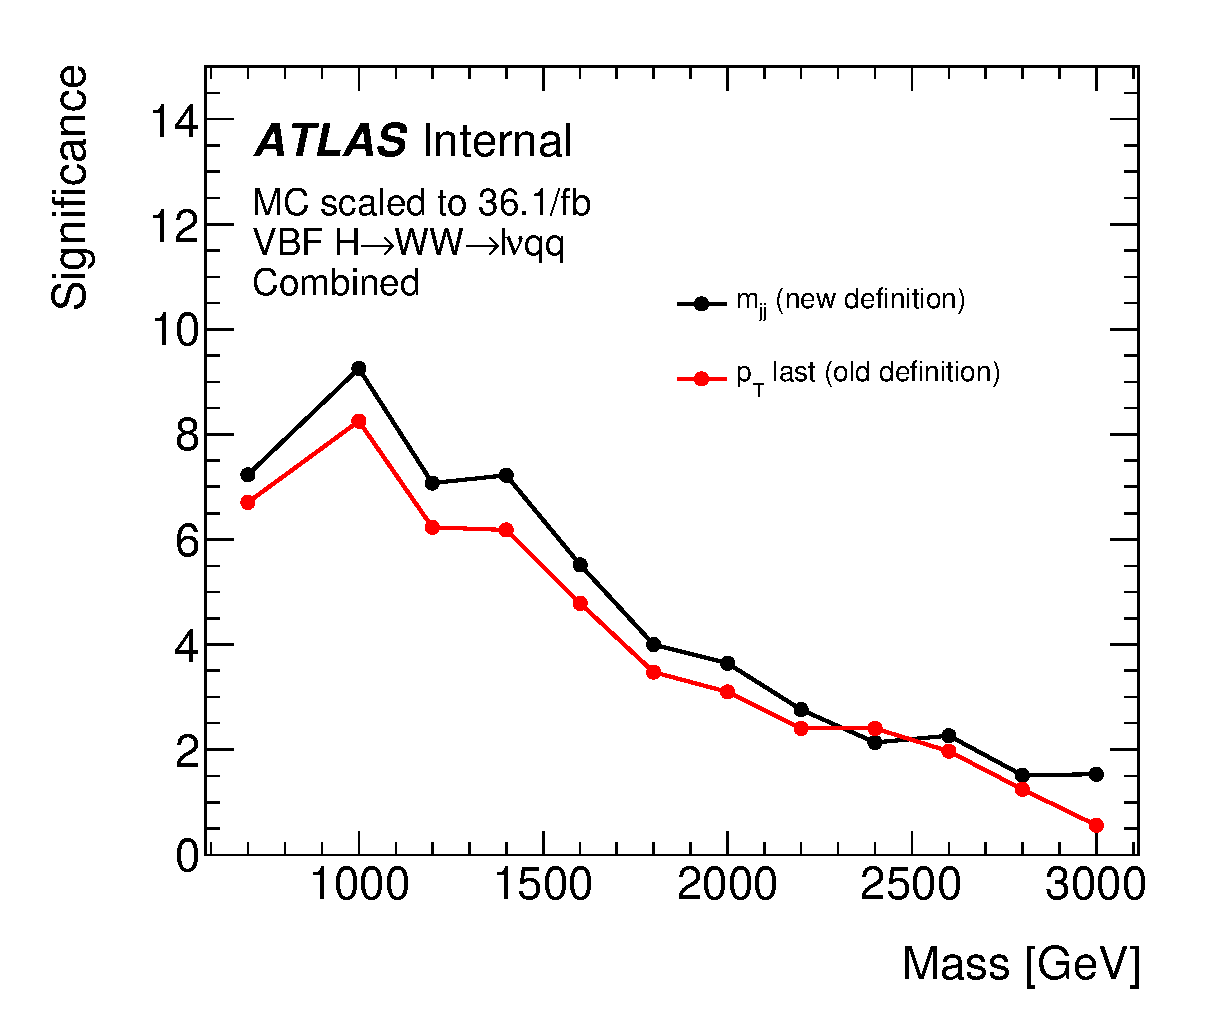
\includegraphics[width=.48\textwidth]{figures/Appendix/opt/mjj_pt/comb_reg_el}\label{fig:mjj_comb:a}}
\subfloat[]{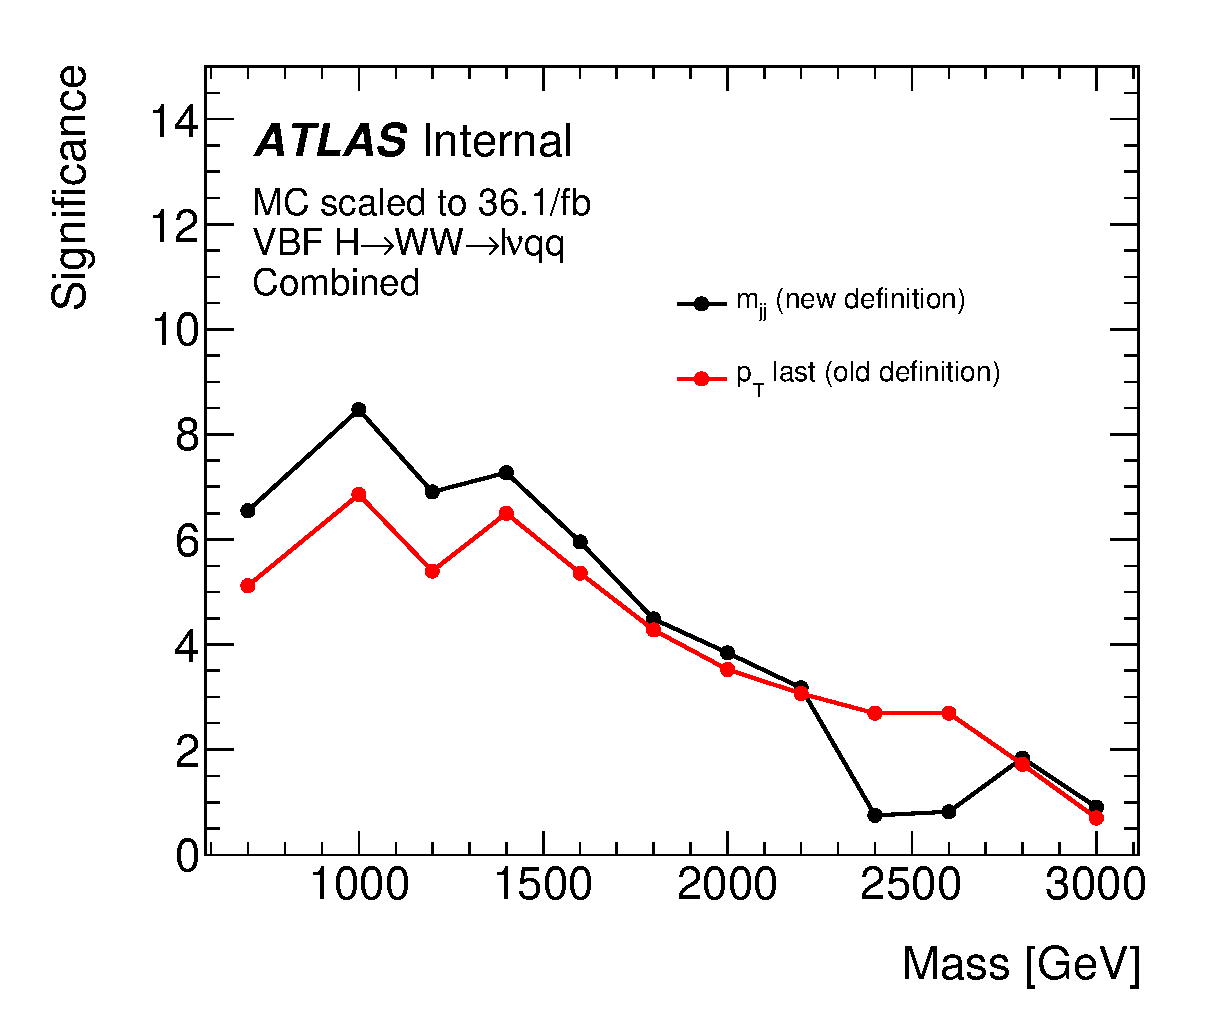
\includegraphics[width=.48\textwidth]{figures/Appendix/opt/mjj_pt/comb_reg_mu}\label{fig:mjj_comb:b}}
\caption[Sensitivity of selection method of vector boson fusion jets in the combined signal region]{Sensitivity of the VBF jet selection in the combined HP+LP SR for the \protect\subref{fig:mjj_comb:a} $e$-channel and \protect\subref{fig:mjj_comb:b} $\mu$-channel. A heavy scalar Higgs (NWA) model was used, for masses between 500\,\GeV\, and 3\,\TeV. For nearly all signal masses, selecting the pair of small-R jets with the largest invariant mass improves the sensitivity.}
\label{fig:mjj_comb}
%\end{figure}
%\begin{figure}[tb]
\centering
\subfloat[]{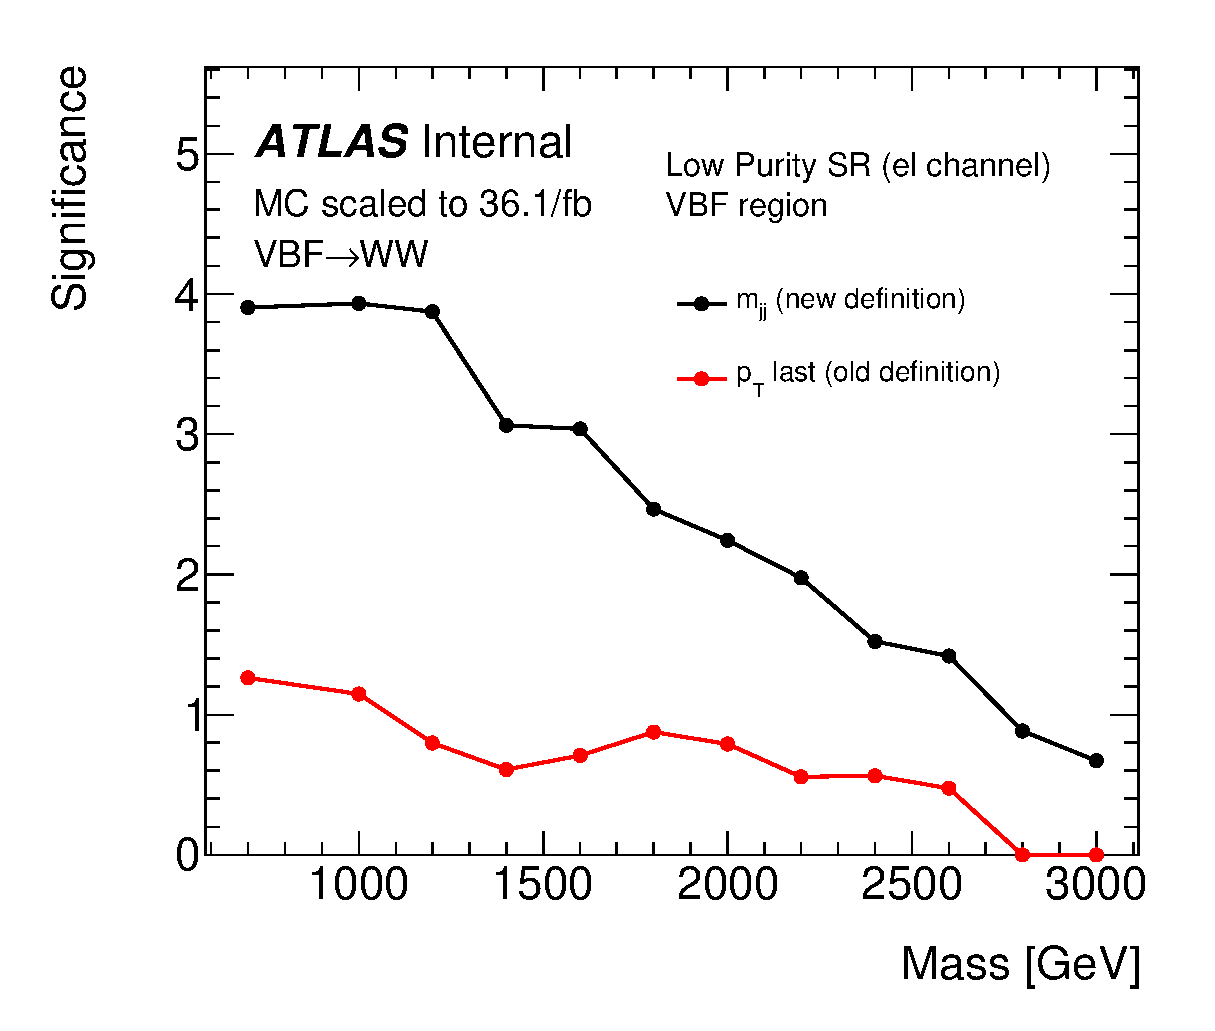
\includegraphics[width=.48\textwidth]{figures/Appendix/opt/mjj_pt/lp/comp_vbf_sig_vbf_reg_el}\label{fig:mjj_lp:a}}
\subfloat[]{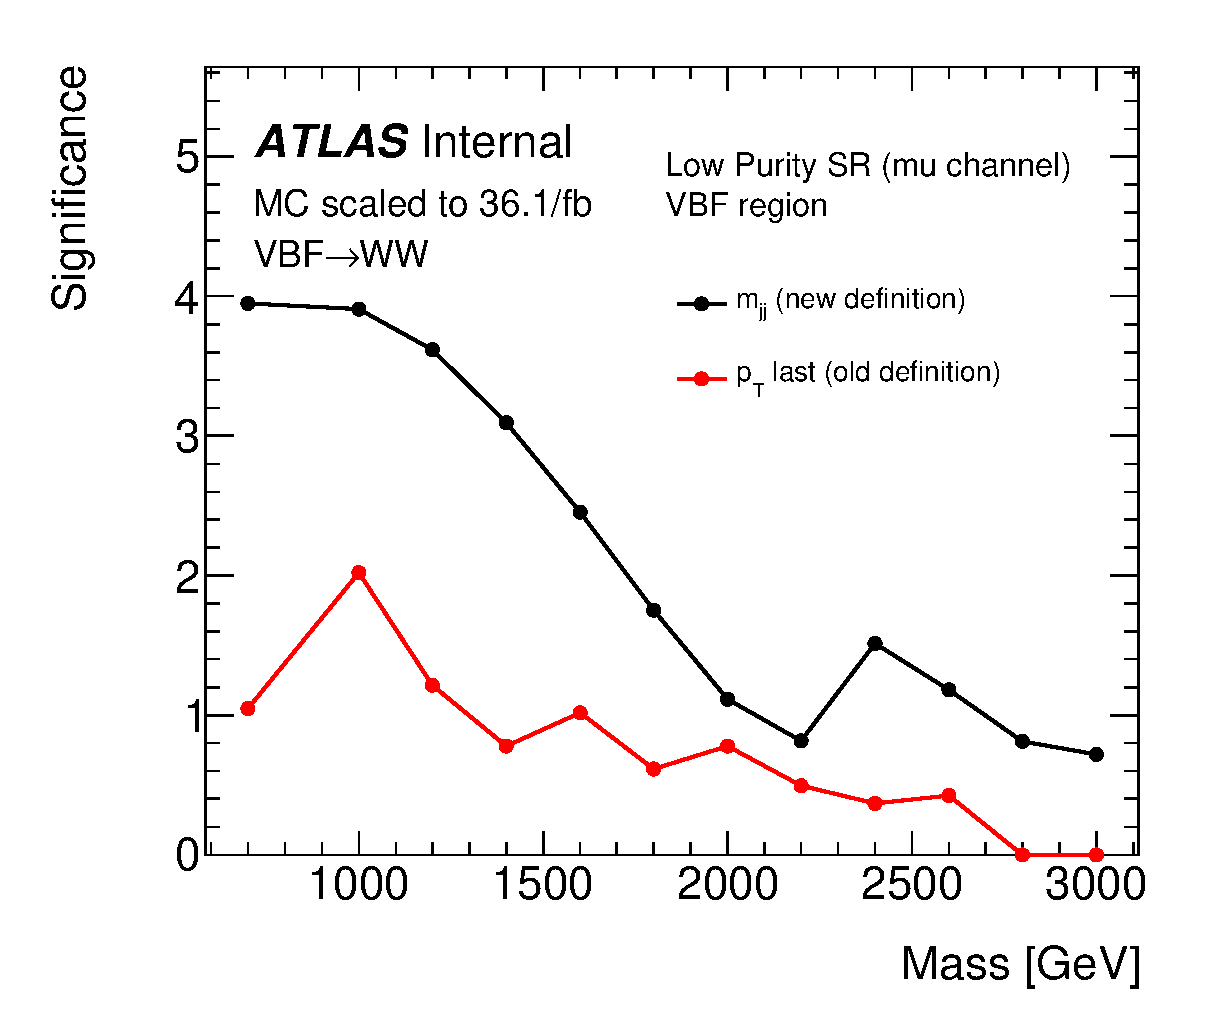
\includegraphics[width=.48\textwidth]{figures/Appendix/opt/mjj_pt/lp/comp_vbf_sig_vbf_reg_mu}\label{fig:mjj_lp:b}}
\caption[Sensitivity of selection method of vector boson fusion jets in the low purity signal region]{Sensitivity of the VBF jet selection in the LP SR for the \protect\subref{fig:mjj_lp:a} $e$-channel and \protect\subref{fig:mjj_lp:b} $\mu$-channel. A heavy scalar Higgs (NWA) model was used, for masses between 500\,\GeV\, and 3\,\TeV. For all signal masses, selecting the pair of small-R jets with the largest invariant mass improves the sensitivity.}
\label{fig:mjj_lp}
\end{figure}


%
\clearpage
\section{Track Assisted Mass}
\label{sec:TAmass}
In this search, the evaluation of large-R jet mass has been updated. Instead of exclusively using calorimeter information to calculate the large-R jet mass, track information can be used to calculate a track-based mass. Since the tracker only measures the momentum of charged particles, a track assisted mass is defined to compensate for the fraction of neutral particles in the jet. The track assisted (TA) mass of the large-R jet is defined by:
\begin{equation}
m_{\textrm{TA}} = m_{{\rm trk}} \times \frac{\pt}{p_{{\rm T,trk}}},
\end{equation}
Here, \pt is the transverse momentum of the large-R jet reconstructed by the calorimeter topo-clusters.  The ratio of the calorimeter-based \pT to the track-based \pT ($p_{{\rm T,trk}}$) compensates for the neutral particle fraction in the jet.

For boosted jets, the particles in the shower may begin overlapping in the calorimeter, degrading the jet mass resolution. The high granularity tracker allows for precise discrimination between nearby tracks. This increased granularity can recover performance loss in the high-\pT region. The response of the track-assisted mass is nearly constant since the \pt of the jet is calibrated, and the tracker gives the momentum scale of the tracks.

The TA mass and calorimeter mass of the large-R jet, near the mass of the $W$ boson, is plotted for simulated jets in~\Fig{\ref{fig:ta_vs_calo_m}}. An HVT $Z$' model is used for signal masses between 500\,\GeV\, and 5\,\TeV. The mass resolution of the large-R jet is defined as $\text{res}(J) = (m_{\text{reco}}-m_{\text{truth}})/m_{\text{truth}}$. The response is determined by fitting the resolution with a gaussian, in slices of $\pT(J)$, and calculating the standard deviation, $\sigma$, of the fit.  The response of the large-R jet mass is plotted as a function of the truth \pT and reconstructed \pT in~\Fig{\ref{fig:ta_vs_calo_res}}.

In this search, a combination of the track assisted mass and calorimeter mass, called the combined mass, is used. The combined mass minimizes the jet mass response in each \pT bin. For lower-\pT, the combined mass is weighted heavily with the calorimeter mass, while in the high-\pT regime, the TA mass is weighted more.
 

\begin{figure}[htbp]
\centering
  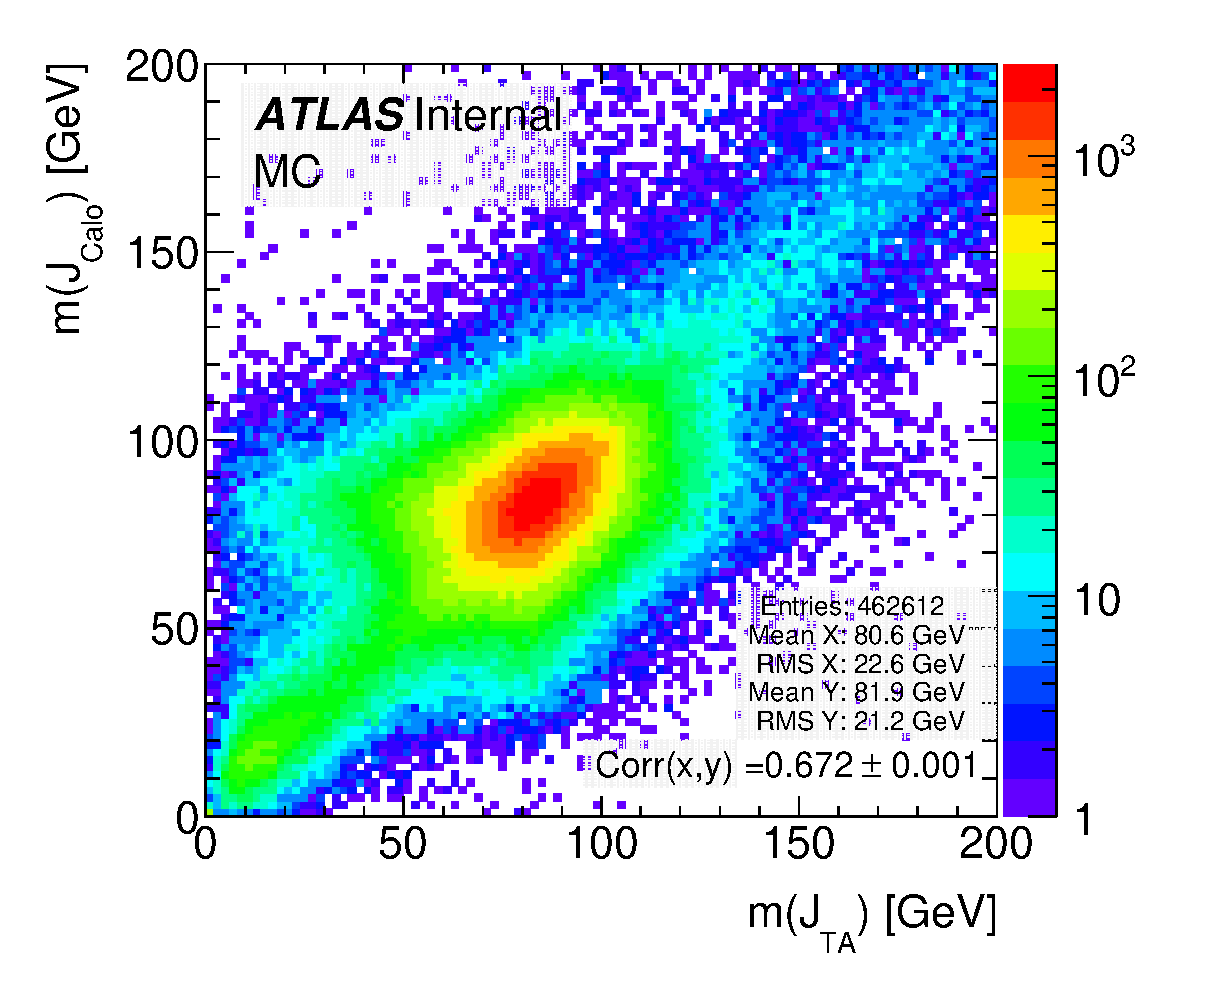
\includegraphics[width=0.7\textwidth]{figures/Appendix/opt/TA/TA_vs_Calo_m}
  \caption[Track assisted mass versus calorimeter mass of the large-R jet]{ The TA mass is plotted against the calorimeter mass of the large-R jet. Simulated HVT $Z'$ signal samples are used for resonance masses between 500\,\GeV and 5\,\TeV.}
  \label{fig:ta_vs_calo_m}
\end{figure}

\begin{figure}[htbp]
\centering
  \subfloat[][\label{fig:ta_vs_calo_resa}]{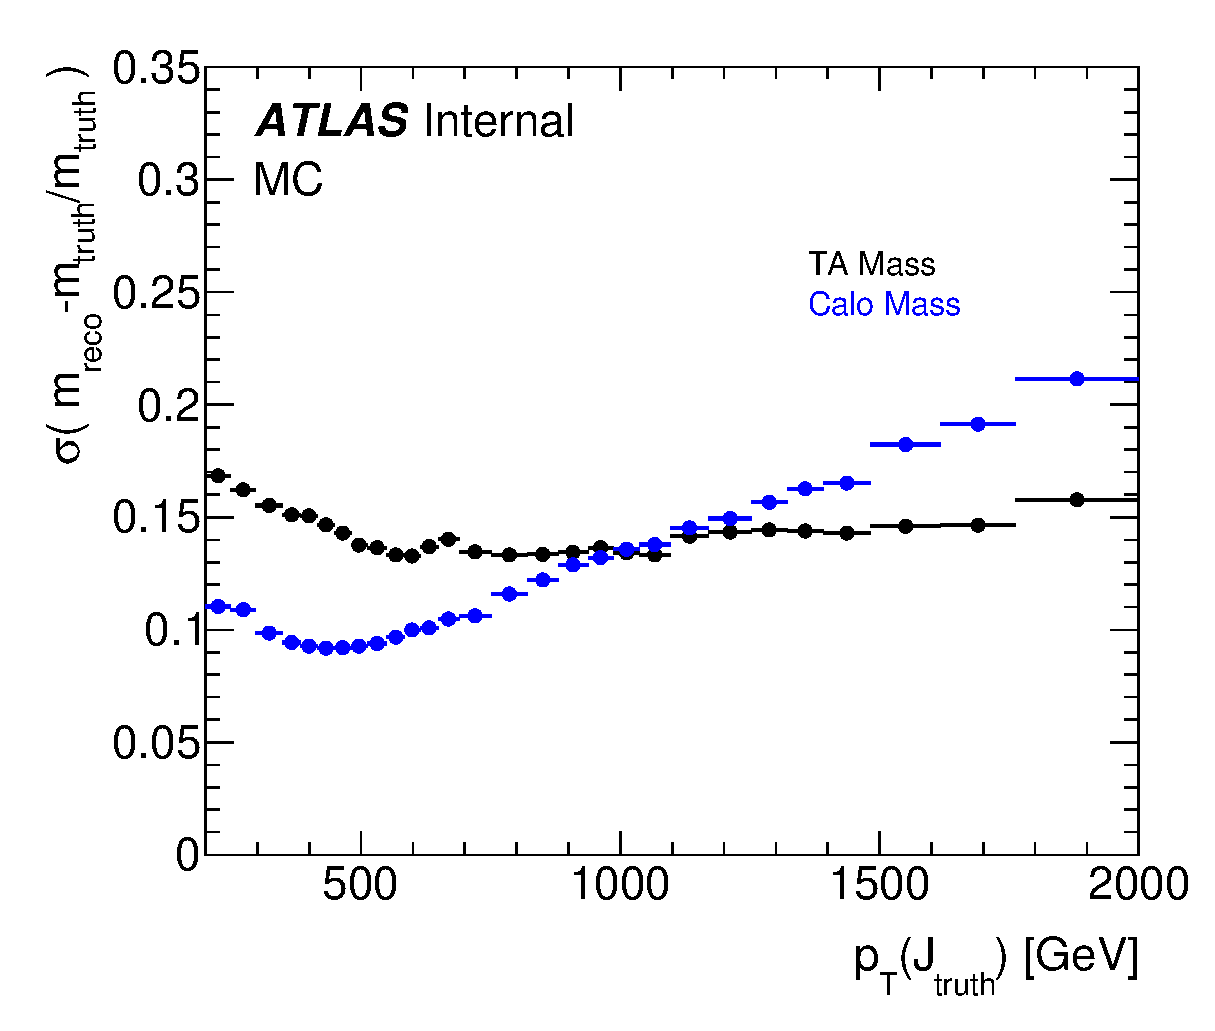
\includegraphics[width=0.48\textwidth]{figures/Appendix/opt/TA/TA_Calo_MassResolution_pttruth}}
  \subfloat[][\label{fig:ta_vs_calo_resb}]{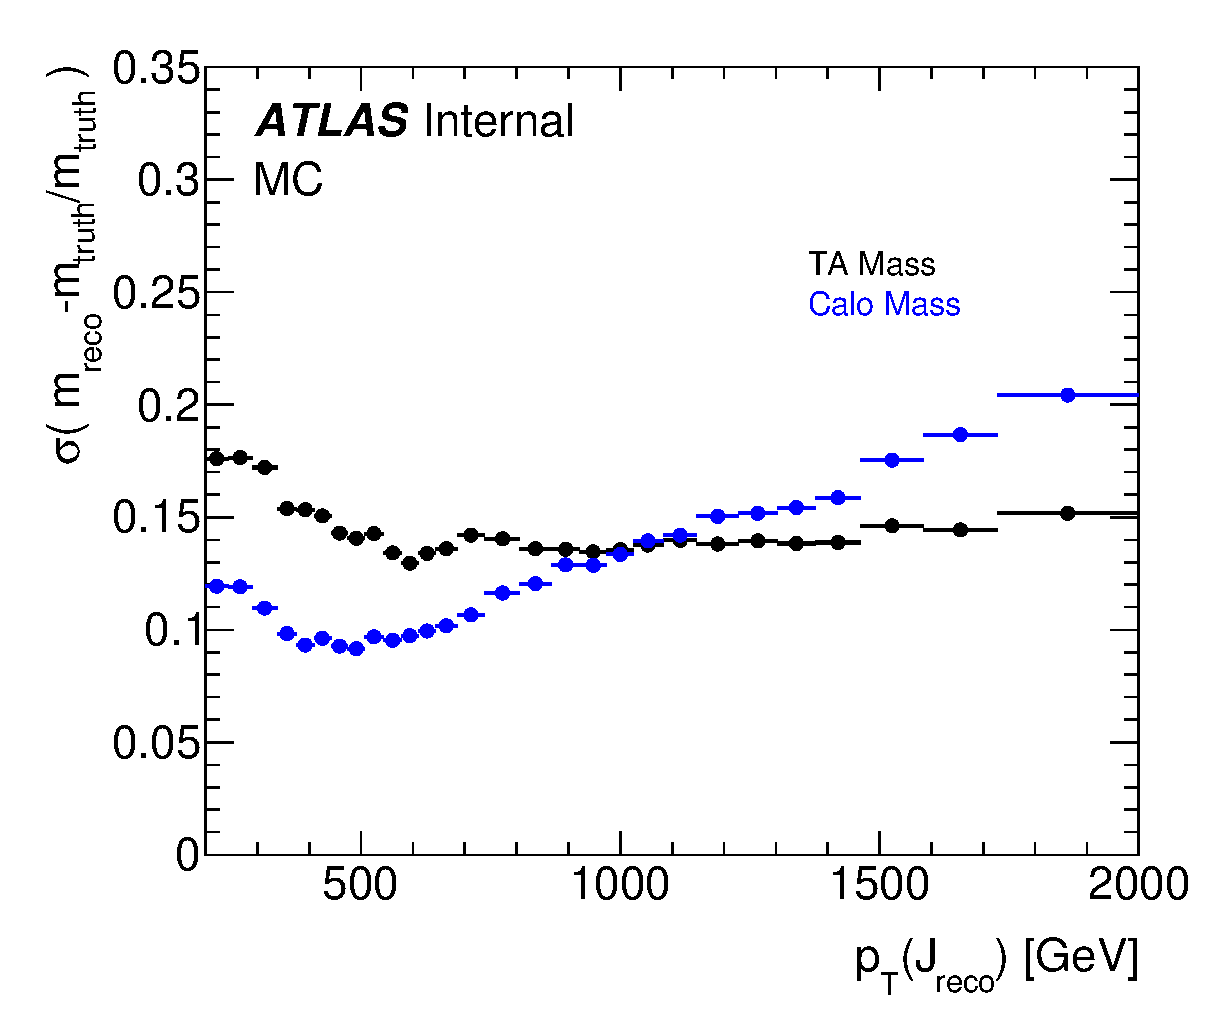
\includegraphics[width=0.48\textwidth]{figures/Appendix/opt/TA/TA_Calo_MassResolution_ptreco}}
  \caption[Response of track assisted mass and calorimeter mass of large-R jet]{ The mass resolution of the large-R jet is calculated as $\text{res}(J) = (m_{\text{reco}}-m_{\text{truth}})/m_{\text{truth}}$. The response is calculated by fitting the resolution, in slices of $p_{\rm T}(J)$, with a Gaussian and the standard deviation, $\sigma$, is measured.
	The response is plotted as a function of ~\subref{fig:ta_vs_calo_resa} $p_{\rm T}(J_{\text{truth}})$ and
	~\subref{fig:ta_vs_calo_resb} $p_{\rm T}(J_{\text{reco}})$. The improved response of the TA mass in the high-\pT region is verified.}
  \label{fig:ta_vs_calo_res}
\end{figure}

